%!TEX root = ../larxxia.tex
\begin{draft}

\section{Establish mathematical truths}
\label{sec:emt}
\secttoc

\begin{comment}
Perhaps do not include in a first version:  needs to be written.
Beezer2015 has a relevant presentation in Proof Techniques, and also sets, in an end-chapter called Preliminaries.
\end{comment}

\begin{quoted}{\index{Weyl, Hermann}Hermann Weyl}
Logic is the hygiene the mathematician practises to keep his ideas healthy and strong.
\end{quoted}

Scientists and engineers develop knowledge using both \idx{induction} and \idx{deduction}.
\begin{itemize}
\item Induction starts with experiments and observations and then infers or fits a formula that generalises measured values---generalises to cases of later use.  
Induction recognises that nature\slash reality is the ultimate arbiter of truth: we humans can discuss as long as we like, but observation\slash experiment must check sanity.

\item Deduction starts from established truths or axioms and invokes logic to discover or suggest new truths.
The logic may be rigorous, or may be based upon `physical' understanding.

\end{itemize}
Mathematicians largely use deduction to construct magnificent edifices of useful knowledge.
But what is constructed is often suggested by, or rests on needs established by, experiment and observation.
Further, deduction is a difficult skill that is prone to error, so this section aims to consolidate the principles used throughout mathematics.


\begin{comment}
experimental mathematics somewhere.
\end{comment}


\subsection{Definitions clarify}
\label{sec:dc}
\index{definition|(}



\begin{quoted}{\index{Hobbes, Thomas}Thomas Hobbes, 1588--1679}
The light of humane minds is perspicuous words, but by exact definitions first snuffed, and purged from ambiguity; reason is the pace \ldots\ And, on the contrary, metaphors, and senseless and ambiguous words are like \emph{ignes fatui} [foolish fire]; and reasoning upon them is wandering amongst innumerable absurdities.
\end{quoted}

Isaac Newton was a great scientist and mathematician.
Among many contributions, his three laws underpin all analysis of the motion of bodies.
One of the most significant parts of the three laws was the clarification of the distinction between velocity and acceleration.
Before Newton, may people had discussed and written about the motion of bodies, but much of that discussion was confused and confounded because different people meant different things by the words they used, and often words meant different things when used by the same person at different times.
It was Newton's careful and consistent distinction between concepts such as velocity and acceleration that empowered scientific progress.

Modern science, engineering and mathematics continues to rely upon good definitions.
Good definitions are essential for providing a precise language that we all understand in order to avoid ``wandering amongst innumerable absurdities''.

\begin{quoted}{Lewis Carroll, 1872}
``When I use a word,'' Humpty Dumpty said, in a rather scornful tone, ``it means just what I choose it to mean---neither more nor less.''
\end{quoted}


\begin{comment}
Sometimes (inconsistently?) use the becomes symbol \index{:=@$:=$}\(:=\)---define here somewhere.  Define \(\in\) and \(\iff\) and \(\implies\) somewhere.  Define sets \(\{\}\) and \(\{:\}\).
\end{comment}

\index{definition|)}



\subsection{Examples suggest or confirm}
\label{sec:egsc}
\index{example|(}

\begin{example}[\idx{Mersenne primes}]
Following the 17th century Minim friar \index{Mersenne, Marin}Marin Mersenne, let's consider the numbers of the form \(2^p-1\) where \(p\)~is prime:
\begin{itemize}
\item \(p=2\) gives \(2^2-1=3\) which is also prime;
\item \(p=3\) gives \(2^3-1=7\) which is also prime;
\item \(p=5\) gives \(2^5-1=31\) which is also prime; and
\item \(p=7\) gives \(2^7-1=127\) which is also prime.
\end{itemize}
This looks like a pattern.
These four cases clearly indicate that all numbers of the form \(2^p-1\), where \(p\)~is prime, are themselves prime.
Unfortunately the pattern of these four cases mislead. 
The pattern is false.
The next case fails as \(2^{11}-1= 2047 =23\times 89\) is not prime.
\end{example}


The moral of this example is that a finite number of cases can \emph{never prove} a universal general truth.
\footnote{\cite{Guy88} gives 35 examples of patterns conjectured on the basis of some cases, and then discusses which generalise and which do not.}
Nonetheless we often use cases as evidence to suggest and support scientific theories, but such scientific theories may be falsified at any time by further evidence.
Although being `falsified' sounds disastrous, often it is not.
Confounding further evidence often just limits the domain of validity of a scientific theory.
For example, Einstein's theory of relativity did not ruin Newtonian mechanics; Einstein's theory just limited Newtonian mechanics to circumstances where speeds are much less than the speed of light.




\begin{example} \label{eg:}
In \script\ the command \verb|factor()|\index{factor()@\texttt{factor()}} returns a list of the prime factors of its integer argument.  
For examples: 
\begin{itemize}
\item \verb|factor(30)| gives \verb|ans = 2 3 5| because \(30=2\cdot3\cdot 5\);

\item \verb|factor(31)| gives \verb|ans = 31| because \(31\)~is a \idx{prime number} and has only itself as a factor (as well as one); and

\item \verb|factor(32)| gives \verb|ans = 2 2 2 2 2| because \(32=2^5\).
\end{itemize}
Use \verb|factor()| to show that, as well as~\(31\) being prime, \(331\), \(3331\), \(33331\), \(333331\) and~\(3333331\) are all prime.
Clearly we conjecture that numbers in this form are always prime.
Let's test this conjecture with the next in the series, \verb|factor(33333331)| indicates it is also prime: the conjecture is working so surely it must be true!
Unfortunately not: for the next in the series \verb|factor(333333331)| finds factors~\(17\) and~\(19,607,843\) so the conjecture fails.
A finite number of successes can only suggest, it cannot establish universal truth.
\end{example}



\index{example|)}






\subsection{Direct proofs}
\label{sec:dp}

\begin{comment}
Currently I only use ``iff'' from \S\ref{sec:iee} and thereafter.
Need to check on \(\iff\) use.
Define set notation, and in, and subset.
\end{comment}
Define \bfidx{iff} and \(\iff\) means ``if and only if''.
and the \idx{converse}.

Proofs often have the structure \(AXA\).
Here \(A\)~denotes some transformation, and/or its reverse, and \(X\)~denotes an key operation that is already established.
One example is the proof of the commutativity of vector addition (\autoref{thm:vecopsa}) which (\(A\))~transforms using the definition of vector addition,  (\(X\))~invokes the commutativity of scalar addition, and lastly, (\(A\))~back transforms into vector addition.
Often there is more than one transformation step: such proofs commonly have the structure~\(ABXBA\), or \(ABCXCBA\), and so on.



\begin{comment}
SEbooklet.pdf has a couple of examples, and a possible approach to describe in understanding proofs.
\end{comment}



\subsection{Proof by contradiction}
\label{sec:pc}
\index{contradiction|(}

\begin{quoted}{\index{Hardy, G.~H.}G.~H. Hardy}
Reductio ad absurdum, which Euclid loved so much, is one of a mathematician's finest weapons.  
It is a far finer gambit than any chess play: a chess player may offer the sacrifice of a pawn or even a piece, but a mathematician offers the game.
\end{quoted}

Introduce \bfidx{pigeonhole principle}.


\index{contradiction|)}


\subsection{Proof by induction}
\label{sec:pi}
\index{induction|(}


\begin{example} \label{eg:}
Consider the sum of the first~\(n\) odd numbers:
\begin{eqnarray*}
n=1,&&1=1^2;\\
n=2,&&1+3=4=2^2;\\
n=3,&&1+3+5=9=3^2;\\
n=4,&&1+3+5+7=16=4^2;\\
n=5,&&1+3+5+7+9=25=5^2.
\end{eqnarray*}
We conjecture that this pattern continues, namely that \(1+3+\cdots+(2n-1)=n^2\) for all positive integer~\(n\).
Use induction to prove this identity.
\begin{solution} 
The identity certainly holds for \(n=1\) (and also for \(n=2,3,4,5\) as seen above).
Induction proceeds by supposing the identity holds for the case \(n=k\) and then proving that then it holds for the next case.
Consider the case \(n=k+1\), then the sum of the first~\((k+1)\) odd numbers is
\begin{eqnarray*}
&&1+3+\cdots+(2k-1)+(2(k+1)-1)\\
&=&k^2+(2k+1)\quad(\text{by induction assumption})\\
&=&k^2+2k+1\\
&=&(k+1)^2\quad(\text{by binomial square}).
\end{eqnarray*}
That is, the sum of the first~\((k+1)\) odd numbers is~\((k+1)^2\).
By induction the identity holds for all~\(n\).
\end{solution}
\end{example}




\index{induction|)}

\sectionExercises



\begin{exercise} \label{ex:} 
Recall the prime numbers less than twenty are \(2,3,5,7,11,13,17,19\)\,.
In this list the number~\(2\) is the only even prime number.
Use contradiction to prove that \(2\) is the only even prime number among all the primes.
\end{exercise}


% selected from \cite{Guy88}

\begin{exercise} \label{ex:} 
Consider the so-called \idx{Fermat numbers} of the form \(2^{2^n}+1\) for integer \(n=0,1,2,\ldots\), namely \(3,5,17,\ldots\)\,.  
Use \verb|factor()|\index{factor()@\texttt{factor()}} in \script\ to show that for small~\(n\) these are \idx{prime number}s.
What is the smallest~\(n\) for which~\(2^{2^n}+1\) fails to be prime?
\answer{\(n=5\)}
\end{exercise}


\begin{exercise} \label{ex:} 
Recall that we define the \idx{factorial} \(n!=n\cdot(n-1)\cdots3\cdot2\cdot1\)\,.
Consider the alternating sums of factorials:
\begin{eqnarray*}
3!-2!+1!&=&5\,;\\
4!-3!+2!-1!&=&19\,;\\
5!-4!+3!-2!+1!&=&101\,;\\
6!-5!+4!-3!+2!-1!&=&619\,.
\end{eqnarray*}
These four alternating sums are all primes: does this continue?
Use \verb|factor()|\index{factor()@\texttt{factor()}} in \script\ to find the smallest case for which the alternating sum is not prime.
\answer{\(9!-8!+\cdots+2!-1!=326981\) is not prime.}
\end{exercise}


\needspace{6\baselineskip}
\begin{exercise} \label{ex:} 
The sequence of \idx{hex numbers} are illustrated below.
\begin{center}
\begin{tikzpicture}
\begin{axis}[title={\normalsize 1}
,tiny,only marks,mark size=0.6ex
,axis lines=none,xmax=4,xmin=-4,ymax=4,ymin=-4,axis equal image]
\addplot+[] table {
   0.0000   0.0000
};
\end{axis}
\end{tikzpicture}\hfil
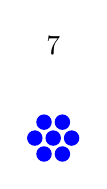
\begin{tikzpicture}
\begin{axis}[title={\normalsize 7}
,tiny,only marks,mark size=0.6ex
,axis lines=none,axis equal image,xmax=4,xmin=-4,ymax=4,ymin=-4]
\addplot+[] table {
  -1.0000   0.0000
  -0.5000   0.8660
  -0.5000  -0.8660
   0.0000   0.0000
   0.5000   0.8660
   0.5000  -0.8660
   1.0000   0.0000
};
\end{axis}
\end{tikzpicture}\hfil
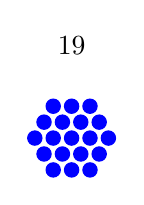
\begin{tikzpicture}
\begin{axis}[title={\normalsize 19}
,tiny,only marks,mark size=0.6ex
,axis lines=none,axis equal image,xmax=4,xmin=-4,ymax=4,ymin=-4]
\addplot+[] table {
  -2.0000   0.0000
  -1.5000   0.8660
  -1.0000   1.7321
  -1.5000  -0.8660
  -1.0000   0.0000
  -0.5000   0.8660
   0.0000   1.7321
  -1.0000  -1.7321
  -0.5000  -0.8660
   0.0000   0.0000
   0.5000   0.8660
   1.0000   1.7321
   0.0000  -1.7321
   0.5000  -0.8660
   1.0000   0.0000
   1.5000   0.8660
   1.0000  -1.7321
   1.5000  -0.8660
   2.0000   0.0000
};
\end{axis}
\end{tikzpicture}\hfil
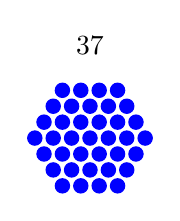
\begin{tikzpicture}
\begin{axis}[title={\normalsize 37}
,tiny,only marks,mark size=0.6ex
,axis lines=none,axis equal image,xmax=4,xmin=-4,ymax=4,ymin=-4]
\addplot+[] table {
  -3.0000   0.0000
  -2.5000   0.8660
  -2.0000   1.7321
  -1.5000   2.5981
  -2.5000  -0.8660
  -2.0000   0.0000
  -1.5000   0.8660
  -1.0000   1.7321
  -0.5000   2.5981
  -2.0000  -1.7321
  -1.5000  -0.8660
  -1.0000   0.0000
  -0.5000   0.8660
   0.0000   1.7321
   0.5000   2.5981
  -1.5000  -2.5981
  -1.0000  -1.7321
  -0.5000  -0.8660
   0.0000   0.0000
   0.5000   0.8660
   1.0000   1.7321
   1.5000   2.5981
  -0.5000  -2.5981
   0.0000  -1.7321
   0.5000  -0.8660
   1.0000   0.0000
   1.5000   0.8660
   2.0000   1.7321
   0.5000  -2.5981
   1.0000  -1.7321
   1.5000  -0.8660
   2.0000   0.0000
   2.5000   0.8660
   1.5000  -2.5981
   2.0000  -1.7321
   2.5000  -0.8660
   3.0000   0.0000
};
\end{axis}
\end{tikzpicture}\hfil
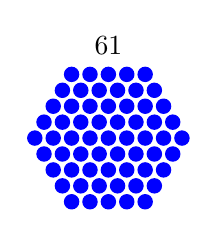
\begin{tikzpicture}
\begin{axis}[title={\normalsize 61}
,tiny,only marks,mark size=0.6ex
,axis lines=none,axis equal image,xmax=4,xmin=-4,ymax=4,ymin=-4]
\addplot+[] table {
  -4.0000   0.0000
  -3.5000   0.8660
  -3.0000   1.7321
  -2.5000   2.5981
  -2.0000   3.4641
  -3.5000  -0.8660
  -3.0000   0.0000
  -2.5000   0.8660
  -2.0000   1.7321
  -1.5000   2.5981
  -1.0000   3.4641
  -3.0000  -1.7321
  -2.5000  -0.8660
  -2.0000   0.0000
  -1.5000   0.8660
  -1.0000   1.7321
  -0.5000   2.5981
   0.0000   3.4641
  -2.5000  -2.5981
  -2.0000  -1.7321
  -1.5000  -0.8660
  -1.0000   0.0000
  -0.5000   0.8660
   0.0000   1.7321
   0.5000   2.5981
   1.0000   3.4641
  -2.0000  -3.4641
  -1.5000  -2.5981
  -1.0000  -1.7321
  -0.5000  -0.8660
   0.0000   0.0000
   0.5000   0.8660
   1.0000   1.7321
   1.5000   2.5981
   2.0000   3.4641
  -1.0000  -3.4641
  -0.5000  -2.5981
   0.0000  -1.7321
   0.5000  -0.8660
   1.0000   0.0000
   1.5000   0.8660
   2.0000   1.7321
   2.5000   2.5981
   0.0000  -3.4641
   0.5000  -2.5981
   1.0000  -1.7321
   1.5000  -0.8660
   2.0000   0.0000
   2.5000   0.8660
   3.0000   1.7321
   1.0000  -3.4641
   1.5000  -2.5981
   2.0000  -1.7321
   2.5000  -0.8660
   3.0000   0.0000
   3.5000   0.8660
   2.0000  -3.4641
   2.5000  -2.5981
   3.0000  -1.7321
   3.5000  -0.8660
   4.0000   0.0000
};
\end{axis}
\end{tikzpicture}
\end{center}
Their partial sums appear to be perfect cubes:
\begin{eqnarray*}
&&1=1^3;\\
&&1+7=8=2^3;\\
&&1+7+19=27=3^3;\\
&&1+7+19+37=64=4^3.
\end{eqnarray*}
Given the \(n\)th~hex number is \(1-3n+3n^2\), use induction to prove that the sum of the first~\(n\) hex numbers is~\(n^3\).
\end{exercise}





\begin{exercise} \label{ex:} 
Recall the prime numbers less than twenty are \(2,3,5,7,11,13,17,19\)\,.
Consider the product of the first~\(n\) of these primes and add one: 
\begin{eqnarray*}
(2)+1&=&3\,;\\
(2\cdot3)+1&=&7\,;\\
(2\cdot3\cdot5)+1&=&31\,;\\
(2\cdot3\cdot5\cdot 7)+1&=&211\,.
\end{eqnarray*}
These four expressions are all primes: does this continue?
Use \verb|factor()|\index{factor()@\texttt{factor()}} in \script\ to find the smallest case for which this product plus one is not prime.
\answer{\((2\cdot3\cdots11\cdot13)+1=30031\) is not prime.}
\end{exercise}




\begin{exercise} \label{ex:} 
\idx{Euler} discovered that the formula \(n^2+n+41\) seemed to always give prime numbers.
For example:
\begin{eqnarray*}
n=0,&&0^2+0+41=41\,;\\
n=1,&&1^2+1+41=43\,;\\
n=2,&&2^2+2+41=47\,;\\
n=3,&&3^2+3+41=53\,;\\
n=4,&&4^2+4+41=61\,.
\end{eqnarray*}
What is the smallest value of integer~\(n\geq0\) such that \(n^2+n+41\) is not prime?
\answer{\(n=41\)}
\end{exercise}






\begin{comment}%{ED498555.pdf}
why, what caused X?
how did X occur?
what-if? what-if-not?
how does X compare with Y?
what is the evidence for X?
why is X important?
\end{comment}





\end{draft}
